\section{Use Case: Coordination of the Heterogeneous Model of a Surveillance Camera System}
\begin{itemize}
	\item This section presents the heterogeneous model of a surveillance camera system. To model the system, we use the TFSM language for modeling the control subsystems (\ie the controller for the camera encoder), whereas for the dataflow aspects of the system we use the Activity language (\ie the encoding algorithms and the battery sensor). In the following, we present each subsystem and how we model them by using the corresponding language. We finish this section by presenting the necessary coordination to get the global system behavior. Then, in the following section, we propose three operators to generate the coordination between these models. 
	
	\item The video surveillance system is composed of a \emph{Battery Sensor} and \emph{Camera Encoder Control}. The camera encoder control takes pictures by using either the \emph{JPEG2000} or \emph{JPG} algorithm depending on the status of the battery. 
	
	\item \todo{to refer the figure of tfsm}
	
	\item The TFSM named \emph{CameraEncoderControl} represents the camera encoder control. When the TFSM model is in state \emph{JPEG2000Encoder}, the JPEG2000 algorithm is used. When in state \emph{JPEGEncoder}, the encoding algorithm is replaced by a mere JPEG algorithm. Each state has a temporal transition that happens every 40 ticks of the \emph{ms} local clock. Each tick of this clock represents one millisecond. Thus, in each state, the camera takes 25 frames per second which corresponds with the standart frame rate for video surveillance. The transition from one state to another is done when either the \emph{BatteryisHigh:occurs} event or the \emph{BatteryisLow:occurs} event occurs, depending on the current state.	
	
		\begin{figure}[h]
			\center
			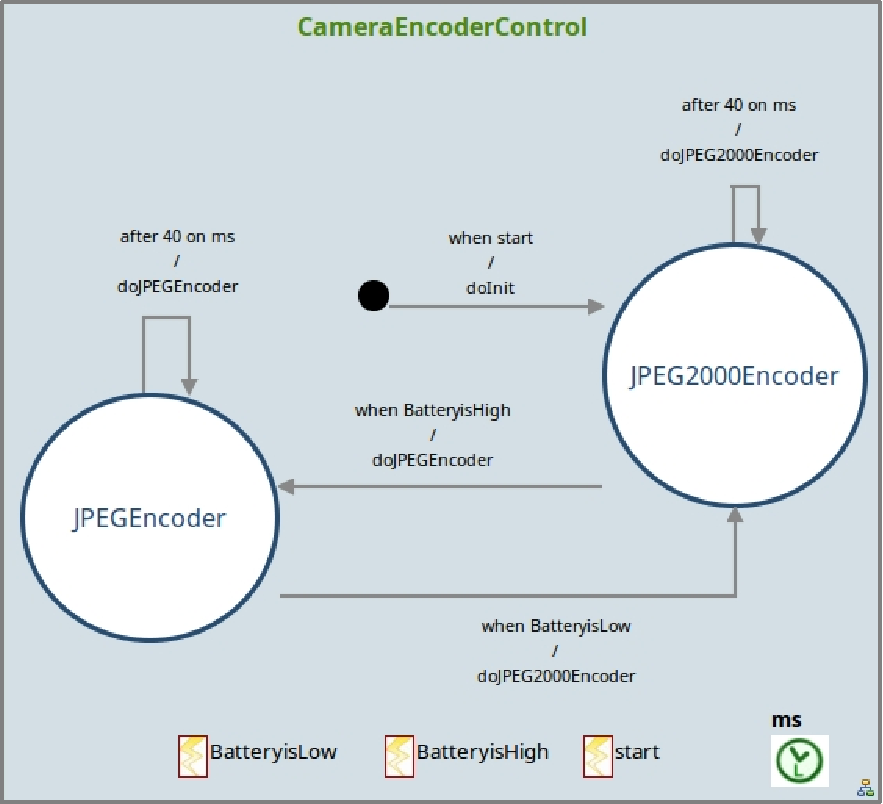
\includegraphics[width=.6\columnwidth]{examples/figs/cameraencodercontrol.pdf}
			\caption{Representation of the Camera Encoder Control by using a TFSM}
			\label{fig:cameramodelencoder}
		\end{figure}
	
	\item In the camera encoder, states are used to represent either the JPEG encoder or the JPEG2000 encoder. Roughly speaking, the JPEG\footnote{http://www.jpeg.org} algorithm encodes a picture by grouping it in blocks which are transformed by a \textit{forward transformation}. Each block of pixels is transformed to frequency coefficient using either a \textit{Fourier transform} (JPEG) or \textit{Wavelet transform} (JPEG2000). The transformed blocks are \textit{quantized} and then passed to a \textit{Run-Length coder} which compress the data. At the end, the block is \textit{transmitted}. We model these algorithms by using the Activity language: the activity named \emph{doJPEG} (see Figure~\ref{fig:dojpeg2000}) represents the JPEG algorithm and the activity named \emph{doJPEG2000} represents the JPEG2000 algorithm . 


	
	\begin{figure}[h]
		\centering
		\begin{minipage}{0.45\textwidth}
			\centering
			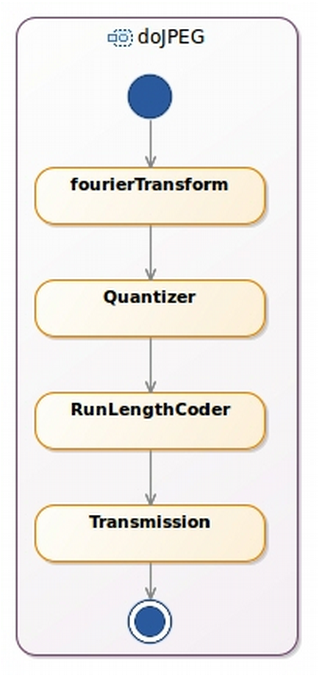
\includegraphics[width=.5\columnwidth]{examples/figs/dojpeg.pdf}
			\caption{Representation of the JPEG encoding algorithm by using activity diagrams}
			\label{fig:dojpeg}
		\end{minipage}\hfill
		\begin{minipage}{0.45\textwidth}
			\centering
			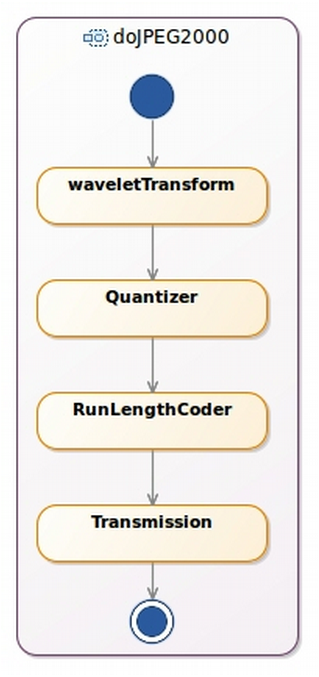
\includegraphics[width=.5\columnwidth]{examples/figs/dojpeg2000.pdf}
			\caption{Representation of the JPEG2000 encoding algorithm by using activity diagrams}
			\label{fig:dojpeg2000}
		\end{minipage}
	\end{figure}
	


	\item \todo{to refer the picture of battery sensor}
	\item The camera control encoder is powered by a battery. When the battery is low, the battery sensor makes the camera use the \emph{JPG} algorithm, thus reducing the quality of the picture but also the energy consumption~\cite{encodingcomparison}. When the battery is high, the JPEG2000 algorithm is used instead. The activity diagrams named \emph{BatterySensor} represents the simple algorithm implemented in the battery sensor. Depending on the status of the battery, the algorithm sends either the signal \emph{BatteryisLow} or \emph{BatteryisHigh}, which correspond with the occurrence of the \mse \emph{BatteryisLow:signalOccurs} and \emph{BatteryisHigh:signalOccurs} respectively.
	
	
			\begin{figure}[h]
				\center
				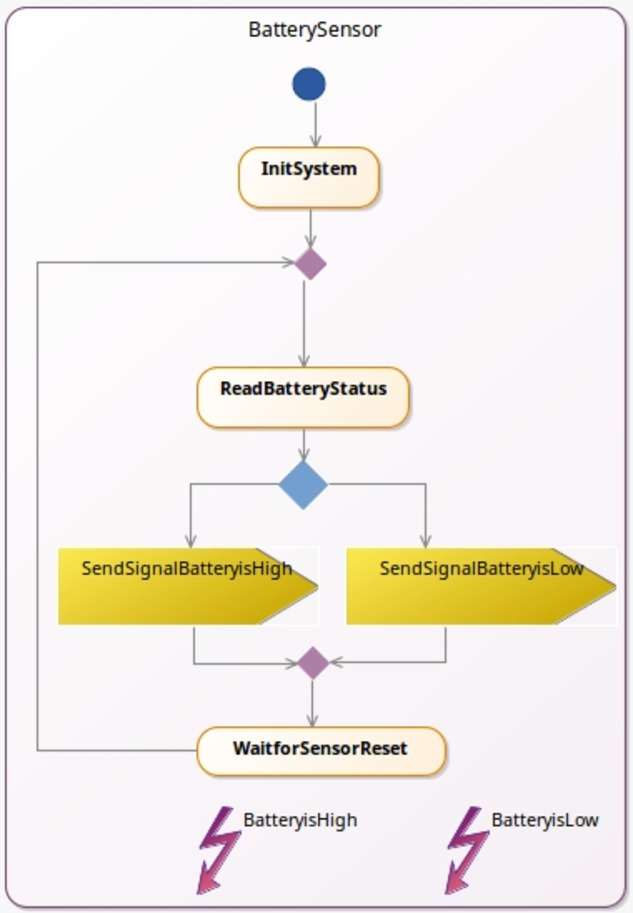
\includegraphics[width=.3\columnwidth]{examples/figs/BatterySensor.pdf}
				\caption{Representation of the Battery Sensor by using activity diagrams}
				\label{fig:batterysensor}
			\end{figure}

	\item To represent the global behavior of the surveillance camera system, we have to specify how these models are coordinated (see Figure~\ref{fig:cameramodel}).
	
	
	
	\begin{figure}
		\center
		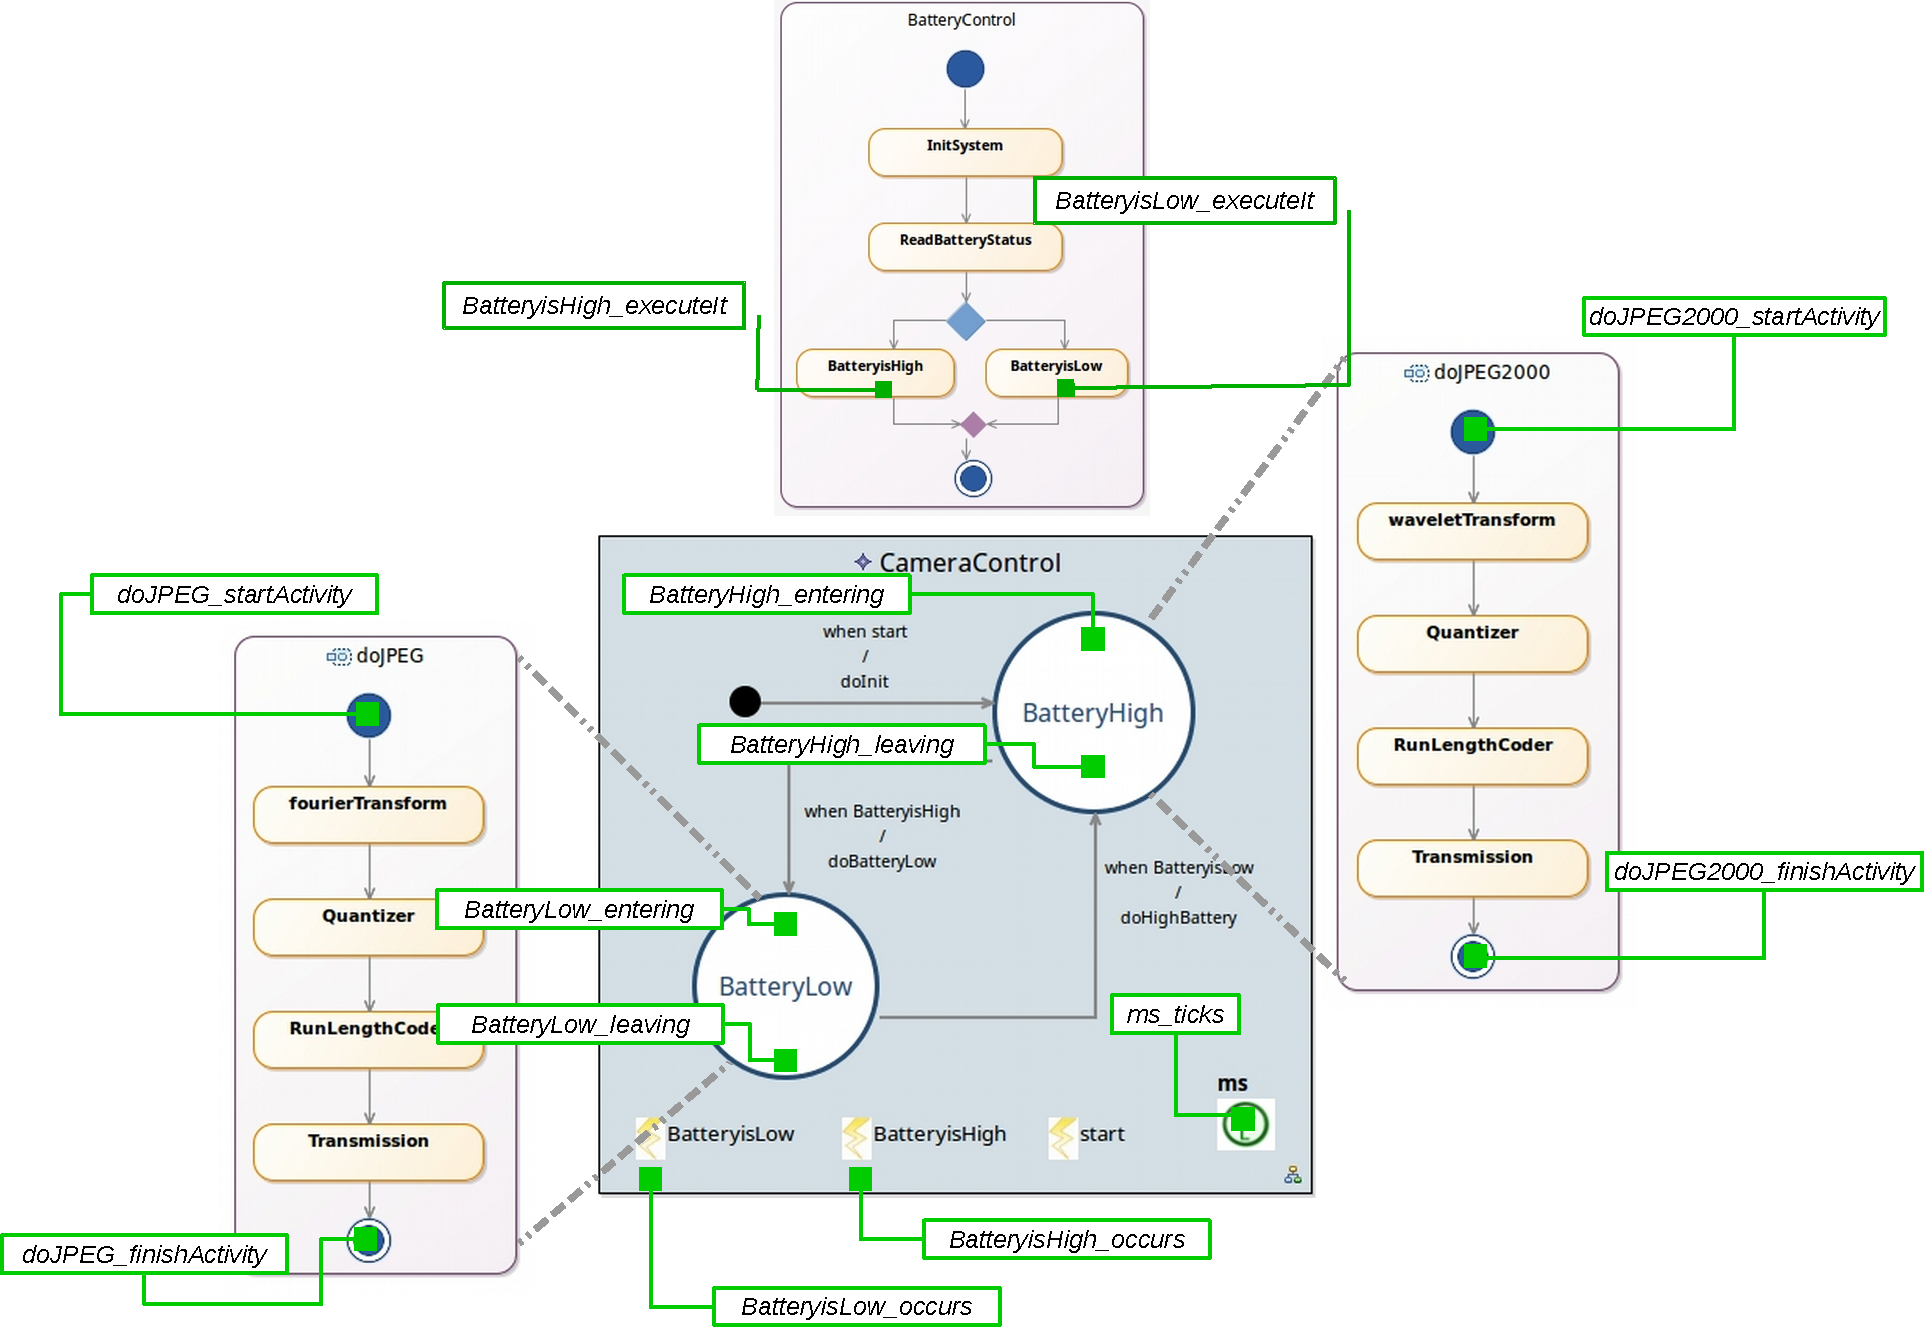
\includegraphics[width=1\columnwidth]{examples/figs/picmodels.pdf}
		\caption{Coordinated model of a surveillance camera system and a partial representation of the model behavioral interface}
		\label{fig:cameramodel}
	\end{figure}
	
	
	\item The activity BatterySensor and the TFSM CameraEncoderControl are coordinated by relying on Signals and FSMEvents. More precisely, the trigger of the signals \emph{BatteryisHigh} and \emph{BatteryisLow} must be synchronized with the occurrences of the FSMEvents \emph{BetteryisHigh} and \emph{BatteryisLow}, \ie synchronization between the \mse \emph{BatteryisHigh:signalOccurs} and \emph{BatteryisHigh:occurs}, and the \mse \emph{BatteryisLow:signalOccurs} and \emph{BatteryisLow:occurs}.
	
	\item The execution of the states of the TFSM CameraEncoderControl must be coordinated with the activities doJPEG and doJPEG2000. To coordinate these models, we have to coordinate the entering and leaving of a state and the execution of the corresponding activity.
	
	\item Finally, to ensure that the camera fulfill the required frames per second, we have to specify how the time in the TFSM elapses during the execution of activities. In other words, we have to specify how the \mse \emph{ms:ticks} is coordinated with the execution of the activities, \eg \emph{doJPEG2000:startActivity} and \emph{doJPEG2000:finishActivity}, \emph{doJPEG:startActivity} and \emph{doJPE:finishActivity}.
	
	\item In this section, we have presented the models that compose a surveillance camera system. To model the system, we used TFSM and Activity languages thus resulting in a heterogeneous model. To represent the global behavior, we have shown how these models need to be coordinated. In the next section, we propose three \bcool operators that specify three coordination patterns between these languages. We then use these operators to generate and execute the coordinated system. 
	
	
	%\begin{itemize}
	%	\item \emph{SyncFSMEventsAndActions}, which specifies a coordination pattern that coordinates Actions and FSMEvents;
	%	\item \emph{startActivityWhenEnter}, which specifies a hierarchical coordination pattern that coordinates the entering and leaving of states and the execution of Activities; 
	%	\item \emph{AtomicActivity}, which specifies a coordination pattern that coordinates the time between TFSMs and Activities. 
	%\end{itemize}
	
	%\item In the following section, we specify these operators in \bcool. For the operator \emph{SyncFSMEventsAndActions}, we rely on the specification presented in chapter~\ref{ch:bcool}.
\end{itemize}


%To represent the global behavior of the surveillance camera system, we have to specify how these models are coordinated. To do so, we propose a set of coordination patterns between the TFSM and Activity languages. In the following, we present the models that must be coordinated together with the pattern to coordinate them. 

%Thus, to coordinate the BatteryControl and the CameraControl, we propose to reuse the operator \emph{SyncFSMEventsAndActions} (see Listing~\ref{lst:bcoolrunningexample}: line 5), which coordinates instances of \dse \emph{occurs} and instances \dse \emph{executeIt} by relying on their names. 

%In this example, we chose the semantics in which entering a specific state of a TFSM model triggers the execution of a given Activity. Then, when leaving a state, several semantic variation points may be chosen. The outgoing transitions from a state can be considered, for instance, as preemptive for the activity model (\ie firing a transition from a state to another preempts the internal activity). Alternatively, the transition can be considered as non-preemptive (\ie the states cannot be left before the associated activity finishes). In our case, we chose non-preemptive transitions. This results that, when the states are reached, the corresponding activity is executed. Then, the state can be left only if the activity has finished. To capture the specification of this coordination pattern, we propose to define a \bcool operator named \emph{startActivityWhenEnter} that implements a hierarchical coordination between states and activity in which transition are non-preemptive.     

%Together with the operator \emph{startActivityWhenEnter}, we propose to specify how the time in the TFSM elapses during the execution of activities. We propose a coordination pattern to coordinate the time between the TFSM and Activity language. In these languages, the time is represented differently. In the TFSM language, each state machine has a \emph{localClock} used to measure the time while the Activity language is untimed. The local clock is a \emph{FSMClock}, which defines a \dse named \emph{ticks} whose occurrences represent a physical time increment. In the Activity language, the duration of activities can be represented as the time between the \dse \emph{startActivity} and \dse \emph{finishActivity}. Thus, to coordinate the time, it is necessary to specify the number of \emph{ticks} of the local clock between the occurrence of the \dse \emph{startActivity} and \emph{finishActivity}. We propose to enforce the execution of the ``internal'' activity to be atomic with respect to the time in the TFSM model. As a result, there are no occurrences of the \dse ticks of the corresponding local clock during the execution of the activity. For example, in the camera, this would result in no occurrences of the \mse \emph{ms:ticks} between the occurrences of the \mse \emph{doJPEG2000:startActivity}, \emph{doJPEG2000:finishActivity}. To capture the specification of this coordination pattern, we propose to define a \bcool operator named \emph{AtomicActivity}, which is also hierarchical but only considers timing aspects.   


 
